Studiamo adesso un'altra tipologia di rivelatori, i cosiddetti scintillatori. Essi sono dei materiali che emettono della luce (detta infatti luce di scintillazione) quando vengono attraversati da una radiazione. I fotoni che vengono emessi in questi materiali non sono tantissimi (o comunque quelli che riusciamo a raccogliere sono veramente pochi) e tipicamente vengono emessi nell'ultravioletto. Alla base di uno scintillatore abbiamo quindi l'emissione di questo flash di luce che ha una durata veramente breve (potrebbe durare anche pochi nanosecondi) e che deriva da transizioni di elettroni, quindi da diseccitazioni degli atomi di questo materiale. Vedremo che, a seconda del tipo di materiale, queste transizioni avvengono tra livelli diversi.

In questo caso ciò che produce un segnale è la raccolta di questa luce. La raccolta di questo segnale in luce ci può dare informazioni sulle particelle, ad esempio sull'energia che è stata depositata da una particella, ma a volte anche sul tipo di particella.

Storicamente, anche se si conoscevano le proprietà di questi materiali, non furono subito applicati nel campo della rivelazione, o comunque non presero particolare piede, bensì venivano sempre utilizzati i rivelatori a gas. Ciò era dovuto ad una semplice questione pratica: questa luce di scintillazione, che è una luce abbastanza fioca ed è pure impercettibile all'occhio umano, veniva inizialmente visualizzata in ambienti scuri attraverso un microscopio. Era quindi una visualizzazione manuale, dunque per niente comoda, pertanto era utilizzata per scopi dimostrativi piuttosto che per scopi di vere e proprie misure. Non appena si svilupparono i primi fotosensori elettronici, strumenti in grado di misurare della luce anche molto debole e trasformarla in un segnale elettrico, gli scintillatori presero il sopravvento divenendo i rivelatori più adoperati.

Esistono diversi tipi di scintillatori, inoltre sono dei materiali che possono essere lavorati in diverse forme dato che ci sono diverse tecniche per la produzione di questi, persino tecniche di estrusione che consistono nel creare degli stampi che si riempiono di questa sostanza ad alta temperatura in forma liquida, la quale poi viene fatta raffreddare ottenendo così lo scintillatore di forma desiderata.

\section{Caratteristiche di uno scintillatore}

\comment{Quali sono i vantaggi degli scintillatori? 

Ogni tipo di scintillatore ha dei vantaggi e degli svantaggi. Diciamo che non esiste lo scintillatore ideale, dipende dal tipo di applicazione. Abbiamo 

\begin{itemize}
   \item una risposta abbastanza lineare in energia, cioè il numero di fotoni che viene prodotto è abbastanza proporzionale all'energia che viene depositata nel materiale e questo è utile perché ci permette di capire quanta energia ha depositato la particella;
   \item Molti di questi materiali hanno tempi di risposta veloci, quindi questa luce viene emessa in tempi abbastanza rapidi, quindi se abbiamo poi un fotosensore e un'elettronica che permettono anche di produrre un segnale veloce allora a quel punto capiamo che sono rivelatori che possono essere utilizzati per il timing, cosa che invece non è quasi mai vera nel caso dei rivelatori a gas, perché i rivelatori a gas tipicamente sono rivelatori abbastanza lenti a causa del fatto che i processi che intervengono sono processi che richiedono una raccolta del segnale che può durare anche centinaia di microsecondi, quindi non li possiamo definire rivelatori veloci a meno che non andiamo a particolari rivelatori come l'MRPC;
   \item Essi permettono di effettuare una discriminazione del tipo di particella che ha inciso, quindi in qualche modo possiamo distinguere tra l'arrivo di una particella $\gamma$ o l'arrivo di una particella carica e questo si fa andando ad analizzare la forma del segnale che viene prodotto.
\end{itemize}
}

In generale, il segnale del rivelatore a scintillazione è in grado di fornire una varietà di informazioni. Purtroppo nessuno scintillatore possiede contemporaneamente tutte le proprietà, quindi la scelta di un particolare tipo rispetto ad un altro dipende da vari fattori e dalla particolare applicazione che richiede di ottimizzare una di queste caratteristiche. Tra le sue caratteristiche più rilevanti ci sono:

\begin{itemize}[leftmargin=0.5cm]
   \item \textit{Sensibilità all'energia}: Al di sopra di una certa energia minima, la maggior parte dei rivelatori a scintillazione si comporta in modo quasi lineare rispetto all'energia depositata, ossia l'emissione di luce di uno scintillatore è direttamente proporzionale all'energia eccitante, cioè all'energia che viene depositata nel materiale e questo è utile perché ci permette di capire quanta energia ha depositato la particella\footnote{Infatti di norma tali materiali vengono collegati ad un fotomoltiplicatore, e poiché è anch'esso un dispositivo lineare (quando utilizzato correttamente!), l'ampiezza del segnale elettrico finale sarà anch'essa proporzionale a questa energia. Questo rende lo scintillatore adatto come spettrometro di energia, anche se non è lo strumento ideale per questo scopo.};
   \item \textit{Risposta temporale rapida}: I rivelatori a scintillazione sono strumenti rapidi, nel senso che i loro tempi di risposta e recupero sono brevi rispetto ad altri tipi di rivelatori. Questa risposta più rapida permette, ad esempio, di ottenere informazioni temporali con maggiore precisione, ossia la differenza di tempo tra due eventi. Inoltre, il breve tempo di recupero consente ai rivelatori a scintillazione di accettare tassi di conteggio più elevati, poiché il tempo morto, ossia il tempo perso in attesa del recupero dello scintillatore, è ridotto. Ecco perché sono rivelatori che possono essere utilizzati per il timing, cosa che invece non è quasi mai vera nel caso dei rivelatori a gas, in quanto quest'ultimi tipicamente sono rivelatori abbastanza lenti a causa del fatto che i processi che intervengono richiedono una raccolta del segnale che può durare anche centinaia di microsecondi, quindi non li possiamo definire rivelatori veloci a meno che non adoperiamo particolari rivelatori come l'MRPC;
   \item \textit{Discriminazione della forma dell'Impulso}: Con certi scintillatori, è possibile distinguere tra diversi tipi di particelle analizzando la forma degli impulsi di luce emessi. Questo è dovuto all'eccitazione di diversi meccanismi di fluorescenza da parte di particelle con diverso potere ionizzante. La tecnica è nota come Pulse Shape Discrimination.
\end{itemize}

Vediamo adesso la struttura base di un rivelatore a scintillazione:

\begin{figure}[H]
   \centering
   \includegraphics[width=\textwidth]{immagini/struttura_base_scintillatore.png}
\end{figure}

Ogni rivelatore basato su scintillatore prevede una parte sensibile di rivelazione, costituita da un blocco di scintillatore, che viene collegato ad un fotosensore, ossia un sensore in grado di misurare questa luce e tradurla in un segnale elettrico che poi può essere inviato in un opportuno sistema di acquisizione.

\subsection{Proprietà ideali di uno scintillatore}
\begin{itemize}[leftmargin=0.5cm]
   \item Alta efficienza di scintillazione (conversione in luce dell'energia depositata con resa fotoni/MeV elevata).\\
   Idealmente vogliamo avere un'alta efficienza di scintillazione, il che vuol dire che se una particella deposita energia, vorremmo che questa energia venisse sfruttata al meglio per produrre fotoni di scintillazione, quindi vorremmo produrre il maggior numero di fotoni in corrispondenza di una data quantità di energia depositata. Tale caratteristica viene quantificata dalla resa in luce, la quale rappresenta il numero di fotoni che vengono prodotti per ogni MeV di energia depositata;
   \item Resa in luce proporzionale all'energia depositata.\\
   Vorremmo anche che la resa in luce fosse proporzionale all'energia depositata, perché in questo modo lo scintillatore può funzionare da rivelatore che misura l'energia della particella depositata;
   \item Spettro della luce di scintillazione adatto ad essere rivelato da opportuni fotosensori.\\
   La luce prodotta dagli scintillatori ricade normalmente negli UV, ma non è sempre così: a volte può essere prodotta una luce sul violetto, ma addirittura anche sul verde o sul rosso, quindi in realtà ogni materiale ha un caratteristico spettro di emissione che ha un'importanza fondamentale perché questa luce deve essere raccolta, dunque è necessario avere un sensore adatto alla luce che viene emessa, altrimenti avremmo un sistema inefficiente perché non siamo in grado di misurare questa luce. Quindi è fondamentale che lo spettro di emissione sia il più possibile vicino alla finestra di lunghezze d'onda a cui il fotosensore è sensibile, quindi bisogna individuare un accoppiamento ottimale in termini di lunghezze d'onda;
   \item Trasparenza alla luce emessa (lunghezza di assorbimento elevata).\\
   Lo scintillatore deve essere trasparente alla luce che emette. Ciò significa che la luce emessa non deve essere riassorbita, perché sennò viene persa. Ciò normalmente si realizza attraverso il drogaggio dei materiali scintillanti.\\
   In termini delle caratteristiche dello scintillatore, questo aspetto equivale a dire che la lunghezza di assorbimento deve essere elevata\footnote{Si veda dopo la definizione di lunghezza di attenuazione.}, dunque la luce che viene emessa deve percorrere lunghi tragitti prima di essere assorbita;
   \item Risposta veloce (tempi di decadimento piccoli).\\
   Non tutti gli scintillatori godono di questa proprietà, però ce ne sono alcuni che hanno una risposta molto veloce e questo ci aiuta non solo per il timing, ma anche per avere delle frequenze di conteggio elevate perché più è breve il segnale prima il rivelatore sarà pronto per misurare una nuova radiazione, pee cui possiamo avere anche delle frequenze di conteggio elevate;
   \item Indice di rifrazione simile a quello del vetro ($n \sim 1.5$)\\
   Ciò è legato al fatto che il rivelatore a scintillazione è sempre costituito dallo scintillatore più il fotosensore, ma non sempre le dimensioni di questi due oggetti sono comparabili, dunque non possiamo semplicemente accostarli l'un l'altro. Sorge pertanto l'esigenza di guidare la luce verso il fotosensore, quindi di creare una sorta di guida di luce che viene realizzata normalmente in plexiglass e che quindi deve avere un indice di rifrazione simile a quello dello scintillatore.
\end{itemize}

\subsection{Tipologie di scintillatori}

Come abbiamo già detto, esistono vari tipi di scintillatore, ognuno dei quali presenta una o più di queste caratteristiche. Sostanzialmente si dividono in due grandi categorie:
\begin{itemize}[leftmargin=0.5cm]
   \item Scintillatori organici, i quali sono composti da molecole contenenti atomi di carbonio, idrogeno e ossigeno. Possono essere di diverse tipologie, ad esempio potremmo avere dei cristalli organici puri, quindi dei materiali che presentano una struttura cristallina, oppure dei materiali amorfi come gli scintillatori plastici. Potremmo anche averli sotto forma di liquido, dunque si parla di liquidi organici;
   \item Scintillatori inorganici, i quali invece possono essere o dei cristalli, o scintillatori a gas o scintillatori a vetro.
\end{itemize}

\section{La luminescenza}

I materiali scintillatori presentano la proprietà nota come luminescenza. I materiali luminescenti, quando esposti a determinate forme di energia, ad esempio luce, calore, radiazioni, ecc., assorbono e riemettono l'energia sotto forma di luce visibile (o invisibile).

\subsection{Cause di luminescenza}

In generale, ci sono tanti materiali che subiscono questi fenomeni che definiamo di luminescenza, la quale si distingue a seconda del tipo di stimolo, perché per emettere della luce il materiale prima deve essere sollecitato, deve ricevere energia, e quindi a seconda della fonte di energia andiamo a distinguere diverse modalità di luminescenza. In base al tipo di stimolo con cui viene indotta la luminescenza, si parla di

\begin{itemize}[leftmargin=0.5cm]
   \item Fotoluminescenza quando il materiale viene stimolato dalla luce;
   \item Termoluminescenza se induciamo la luminescenza attraverso il calore\footnote{Un'applicazione di tale fenomeno sono le tecniche di datazione basate sulle termoluminescenze, che consistono nel far emettere materiali che hanno immagazzinato nel tempo elettroni in delle trappole i quali vengono poi liberati attraverso il riscaldamento del materiale. In base a quanta luce viene emessa si ricava il numero di elettroni che sono stati intrappolati nel tempo, deducendo così quanto tempo è trascorso e quindi si risale all'età del campione.};
   \item Sonoluminescenza attraverso un'onda sonora;
   \item Elettroluminescenza attraverso energia elettrica;
   \item Triboluminescenza attraverso deformazioni meccaniche del materiale;
   \item Chemiluminescenza attraverso reazioni chimiche;
   \item Bioluminescenza attraverso organismi viventi, tipicamente quelli che vivano a vedere nel mare, e allora si parla di bioluminescenza.
\end{itemize}

\subsection{Il processo di scintillazione}
Nel caso degli scintillatori il processo che avviene è la scintillazione, cioè emissione di fotoni a seguito di eccitazione di atomi o molecole che viene indotta da radiazione. Nel caso in esame lo stimolo è quindi una radiazione che può essere una particella o una radiazione $\gamma$. Se guardiamo in generale le caratteristiche della luce emessa per scintillazione possiamo distinguere diverse componenti:
\begin{figure}[H]
   \centering
   \includegraphics[width=0.6\textwidth]{immagini/tipi_di_luce.png}
\end{figure}
In generale si nota che la luce emessa diminuisce nel tempo e lo fa esponenzialmente. In altre parole, l'evoluzione nel tempo del flash di luce prodotto ha un andamento esponenziale decrescente; inoltre la pendenza di questo esponenziale dipende dalle transizioni che hanno dato luogo a questa luce.

Possiamo evidenziare diverse componenti della luce emessa:

\begin{itemize}[leftmargin=0.5cm]
   \item Abbiamo una componente prompt, cioè veloce, che è la luce di fluorescenza. Questa viene emessa con tempi caratteristici molto brevi, come dimostra la pendenza maggiore nel grafico, esaurendosi in pochi nanosecondi. Questa è la componente più veloce e anche quella più importante poiché dà il contributo maggiore;
   \item Si possono avere anche fenomeni di fosforescenza, che tipicamente sono dei fenomeni più lenti, dell'ordine dei millisecondi o secondi. Tale fenomeno è tipico dei materiali che dopo essere stati illuminati continuano a emettere luce di fosforescenza anche dopo diversi secondi\footnote{Come dice il Leo, "Se la riemissione avviene immediatamente dopo l'assorbimento o, più precisamente, entro $10^{-8} \; \rm s$ (che è all'incirca il tempo necessario per le transizioni atomiche), il processo viene solitamente chiamato fluorescenza. Tuttavia, se la riemissione è ritardata perché lo stato eccitato è metastabile, il processo è chiamato fosforescenza o luminescenza residua. In questi casi, il tempo di ritardo tra l'assorbimento e la riemissione può durare da pochi microsecondi a diverse ore, a seconda del materiale.".};
   \item Si potrebbe avere anche una fluorescenza ritardata, cioè un'emissione con dei tempi caratteristici che sono ancora maggiori, ma hanno lunghezze d'onda simili a quelle della emissione di fluorescenza.
\end{itemize}

%Ognuno di questi ha dei vantaggi e degli svantaggi, che approfondiremo nel seguito.

\section{Scintillatori organici}

\subsection{Processo di scintillazione negli scintillatori organici}

Cerchiamo di capire quali sono i principi attraverso cui abbiamo l'emissione di luce di scintillazione negli scintillatori organici.\footnote{La spiegazione dei fenomeni che portano alla produzione di luce sia negli scintillatori organici che in quelli inorganici è stata presa dal Knoll. Sebbene più approfondite, ho preferito riportare queste perché esposte in maniera più esaustiva.}

Osserviamo innanzitutto che questa luce di scintillazione è associata a transizioni di elettroni di valenza liberi, i quali sono degli elettroni che appartenono alla molecola ma non sono associati a uno specifico atomo di questa. Andiamo allora a vedere i livelli che può occupare un elettrone di questo tipo.

Una vasta categoria di scintillatori organici pratici è basata su molecole organiche con determinate proprietà di simmetria che danno origine a ciò che è noto come una struttura elettronica "$\pi$". I livelli di energia elettronici $\pi$ di una tale molecola sono illustrati nella seguente figura:
\begin{figure}[H]
   \centering
   \includegraphics[width=0.7\textwidth]{immagini/Livelli_energetici_scintillatori_organici.png}
\end{figure}
L'energia può essere assorbita eccitando la configurazione elettronica in uno qualsiasi dei numerosi stati eccitati. In figura è riportata una serie di stati di singoletto (spin totale pari a 0), etichettata come $S_0, S_1, S_2, \ldots$ ed è anche mostrato un insieme di livelli elettronici detti stati di tripletto (spin totale pari a 1), etichettati come $T_1, T_2, T_3, \ldots$\footnote{Queste due tipologie di stati sono state messe una accanto all'altra soltanto per evitare di creare confusione, ovviamente ciò che conta è la loro posizione rispetto alla direzione verticale, in cui è riportata l'energia.}

Per le molecole di interesse come quelle degli scintillatori organici, il gap energetico tra $S_0$ e $S_1$ è di 3 o 4 eV, mentre lo spazio tra gli stati superiori è solitamente leggermente più piccolo. Ognuna di queste configurazioni elettroniche è ulteriormente suddivisa in una serie di livelli con spaziature molto più fini che corrispondono a vari stati vibrazionali della molecola, associati a tali moti. La spaziatura tipica di questi livelli è dell'ordine di 0,15 eV. Spesso viene aggiunto un secondo pedice per distinguere questi stati vibrazionali, e il simbolo $S_{00}$ rappresenta lo stato vibrazionale più basso dello stato elettronico fondamentale.

Poiché lo spazio tra gli stati vibrazionali è grande rispetto all'energia termica media ($0.025$ eV), quasi tutte le molecole a temperatura ambiente si trovano nello stato $S_{00}$. Nella figura di sopra l'assorbimento di energia da parte della molecola è rappresentato dalle frecce che puntano verso l'alto. Nel caso di uno scintillatore, questi processi rappresentano l'assorbimento di energia cinetica da una particella carica o da un $\gamma$ che passa nelle vicinanze. Gli stati elettronici di singoletto superiori, che sono stati eccitati, vengono diseccitati rapidamente (in tempi dell'ordine di picosecondi) allo stato elettronico $S_1$ tramite un processo detto di conversione interna, nel quale gli elettroni scendono verso tale stato senza produzione di radiazione. Inoltre, qualsiasi stato con un'energia vibrazionale in eccesso (come $S_{11}$ o $S_{12}$) non è in equilibrio termico con i suoi vicini e perde rapidamente quell'energia vibrazionale.

Pertanto, l'effetto netto del processo di eccitazione in un semplice cristallo organico è quello di produrre, dopo un periodo di tempo trascurabilmente breve, una popolazione di molecole eccitate nello stato $S_{10}$. La principale luce di scintillazione (o fluorescenza rapida) viene emessa nelle transizioni tra questo stato $S_{10}$ e uno degli stati vibrazionali dello stato elettronico fondamentale. Queste transizioni sono indicate in figura dalle frecce rivolte verso il basso. Se $\tau$ rappresenta il tempo di decadimento della fluorescenza per il livello $S_{10}$, allora l'intensità della fluorescenza rapida in un istante $t$ successivo all'eccitazione dovrebbe essere semplicemente
\begin{equation*}
   I=I_0 e^{-\frac{t}{\tau}}
\end{equation*}
Nella maggior parte degli scintillatori organici, $\tau$ è di pochi nanosecondi, e quindi la componente di scintillazione rapida è relativamente veloce.

La vita media del primo stato di tripletto $T_1$ è caratteristicamente molto più lunga di quella dello stato singoletto $S_1$. Attraverso una transizione chiamata "intersystem crossing", alcuni stati di singoletto eccitati possono essere convertiti in stati di tripletto. La vita media di $T_1$ può essere anche di $10^{-3}$ s, e la radiazione emessa in una diseccitazione da $T_1$ a $S_0$ è quindi un'emissione luminosa ritardata etichettata come fosforescenza. Poiché $T_1$ si trova sotto $S_1$, la lunghezza d'onda di questo spettro di fosforescenza sarà maggiore rispetto a quella dello spettro di fluorescenza. Mentre si trovano nello stato $T_1$, alcune molecole possono essere eccitate termicamente di nuovo nello stato $S_1$ e successivamente decadere tramite la fluorescenza normale. Questo processo rappresenta l'origine della fluorescenza ritardata talvolta osservata negli scintillatori organici.

\subsection{Emissione e assorbimento}

Lo schema dei livelli può essere utilizzato anche per spiegare perché gli scintillatori organici possono essere trasparenti alla propria emissione fluorescente. La lunghezza delle frecce rivolte verso l'alto corrisponde a quelle energie dei fotoni che saranno fortemente assorbite nel materiale. Poiché tutte le transizioni di fluorescenza rappresentate dalle frecce rivolte verso il basso (eccetto $S_{10}-S_{00}$, che è l'unico caso in cui la radiazione può essere riassorbita) hanno un'energia inferiore al minimo richiesto per l'eccitazione, c'è pochissima sovrapposizione tra gli spettri di assorbimento ottico e di emissione (spesso chiamata "spostamento di Stokes" o Stokes shift), e di conseguenza c'è poco auto-assorbimento della fluorescenza.

Possiamo vedere un esempio di questi spettri per uno scintillatore organico nel seguente grafico qualitativo, dove notiamo come lo spettro di emissione si trovi a lunghezze d'onda maggiori rispetto a quello in assorbimento:

\begin{minipage}{0.465\textwidth}
   \begin{figure}[H]
      \centering
      \includegraphics[width=\textwidth]{immagini/spettro_assorbimento_e_emissione_scintillatori_organici.png}
   \end{figure}
\end{minipage}
\begin{minipage}{0.53\textwidth}
   \vspace{0.3cm}Il fatto che la luce assorbita si trovi per $\lambda$ minori significa che le energie che vengono assorbite sono maggiori (in quanto $E=h\nu=\frac{c}{\lambda}$), in accordo con quanto detto prima.\\Notiamo inoltre che tra i due spettri c'è un overlap, cioè una sovrapposizione. Ciò vuol dire che la luce emessa potrebbe essere riassorbita, però nella pratica si cerca di mantenere tale overlap il più piccolo possibile.
\end{minipage}

\begin{esempio}
   Andiamo adesso a guardare uno spettro più quantitativo.
   In figura possiamo vedere lo spettro di uno scintillatore plastico:

   \begin{minipage}{0.39\textwidth}
      \begin{figure}[H]
         \centering
         \includegraphics[width=\textwidth]{immagini/esempio_spettro_scintillatore organico.png}
      \end{figure}
   \end{minipage}
   \hfill
   \begin{minipage}{0.6\textwidth}
      \vspace{1cm}Il numero posto sopra è dovuto al fatto che, solitamente, per identificare tali scintillatori si adoperano delle sigle che derivano dalle case produttrici. 
      Guardando i valori di lunghezza d'onda notiamo che ricadiamo nella regione a cavallo tra il violetto e l'ultravioletto, addirittura la coda destra del grafico cade verso la componente azzurra. Normalmente questi spettri di emissione presentano dei picchi, per cui spesso alcuni dati che si trovano nelle tabelle (ad esempio l'indice di rifrazione del materiale, il quale dipende dalla lunghezza d'onda) si riferiscono ai valori che si hanno in corrispondenza della lunghezza d'onda del picco.
   \end{minipage}
\end{esempio}

\section{Scintillatori inorganici}


\subsection{Meccanismo di scintillazione nei cristalli inorganici}
Mentre per gli scintillatori organici l'emissione è legata a transizioni tra livelli della molecola, in quelli inorganici il meccanismo di scintillazione dipende dagli stati energetici determinati dal reticolo cristallino del materiale.
\begin{figure}[H]
   \centering
   \includegraphics[width=0.75\textwidth]{immagini/Livelli_energetici_scintillatori_inorganici.png}
\end{figure}
Come mostrato nella figura sopra, gli elettroni hanno a disposizione solo bande di energia discrete nei materiali classificati come isolanti o semiconduttori. La banda inferiore, chiamata banda di valenza, rappresenta quegli elettroni che sono essenzialmente legati ai siti del reticolo, mentre la banda di conduzione rappresenta quegli elettroni che hanno sufficiente energia per essere liberi di migrare attraverso il cristallo. Esiste una banda intermedia di energie, chiamata banda proibita, nella quale gli elettroni non possono mai essere trovati nel cristallo puro.

L'assorbimento di energia può provocare la promozione di un elettrone dalla sua posizione normale nella banda di valenza oltre il gap, fino alla banda di conduzione, lasciando una lacuna nella banda di valenza normalmente piena\footnote{La professoressa afferma che si tratta di un processo di ionizzazione. Tale fenomeno può essere visto in tal modo poiché implica la rimozione di un elettrone dal suo stato legato, creando una lacuna (carica positiva) e un elettrone libero nella banda di conduzione, ma è alquanto improprio perché l'elettrone non viene veramente liberato.}. Nel cristallo puro, il ritorno dell'elettrone alla banda di valenza con l'emissione di un fotone è un processo inefficiente. Inoltre, le larghezze tipiche del gap sono tali che il fotone risultante avrebbe un'energia troppo elevata per rientrare nello spettro visibile.

Per aumentare la probabilità di emissione di fotoni visibili durante il processo di diseccitazione, si aggiungono comunemente piccole quantità di impurità agli scintillatori inorganici. Queste impurità, chiamate \textit{attivatori}, creano siti speciali nel reticolo in cui la normale struttura delle bande energetiche viene modificata rispetto a quella del cristallo puro. Di conseguenza, verranno creati stati energetici all'interno del gap proibito, attraverso i quali l'elettrone può diseccitarsi ritornando alla banda di valenza. Poiché l'energia è inferiore a quella dell'intero gap proibito, questa transizione può ora dare origine a un fotone visibile e quindi costituire la base del processo di scintillazione. Questi siti di diseccitazione sono chiamati centri di luminescenza o centri di ricombinazione. La loro struttura energetica nel reticolo cristallino ospite determina lo spettro di emissione dello scintillatore.

Una particella carica che attraversa il mezzo di rivelazione formerà un gran numero di coppie elettrone-lacuna create dalla promozione degli elettroni dalla banda di valenza a quella di conduzione. La lacuna positiva si sposterà rapidamente verso il sito di un attivatore e lo ionizzerà, poiché l'energia di ionizzazione dell'impurità sarà inferiore a quella di un sito tipico del reticolo. Nel frattempo, l'elettrone è libero di migrare attraverso il cristallo e lo farà fino a incontrare un tale attivatore ionizzato. A questo punto l'elettrone può cadere nel sito dell'attivatore, creando una configurazione neutra che può avere i propri stati energetici eccitati. Questi stati sono illustrati nella figura come linee orizzontali all'interno del gap proibito. Se lo stato dell'attivatore che si forma è una configurazione eccitata con una transizione consentita verso lo stato fondamentale, la sua diseccitazione avverrà molto rapidamente e con alta probabilità di emissione di un fotone corrispondente. Se l'attivatore è scelto correttamente, questa transizione può avvenire nel campo di energia visibile (cioè si produrrà luce visibile). I tempi di vita tipici per tali stati eccitati sono dell'ordine di 30-500 ns. Poiché il tempo di migrazione per l'elettrone è molto più breve, tutte le configurazioni di impurità eccitate si formano essenzialmente allo stesso tempo e successivamente si disecciteranno con l'emivita caratteristica dello stato eccitato. È quindi il tempo di decadimento di questi stati a determinare le caratteristiche temporali della luce di scintillazione emessa. Alcuni scintillatori inorganici possono essere adeguatamente caratterizzati da un singolo tempo di decadimento o da un semplice esponenziale, anche se spesso si osservano comportamenti temporali più complessi.

Esistono processi che competono con quello appena descritto. Ad esempio, l'elettrone, una volta arrivato al sito dell'impurità, può creare una configurazione eccitata la cui transizione allo stato fondamentale è proibita. Tali stati richiedono quindi un incremento aggiuntivo di energia per elevarli a uno stato più elevato da cui la diseccitazione verso lo stato fondamentale è possibile. Una fonte di questa energia è l'eccitazione termica, e la componente lenta risultante della luce è chiamata fosforescenza. Spesso può essere una fonte significativa di luce di fondo o "afterglow" negli scintillatori.

Esiste una terza possibilità quando un elettrone viene catturato nel sito di un attivatore. Alcune transizioni senza radiazione sono possibili tra alcuni stati eccitati formati dalla cattura dell'elettrone e lo stato fondamentale, nel qual caso non si produce alcun fotone visibile. Tali processi sono chiamati quenching e rappresentano meccanismi di perdita nella conversione dell'energia della particella in luce di scintillazione.

In alternativa alla migrazione indipendente dell'elettrone e della lacuna descritta sopra, la coppia può invece migrare insieme in una configurazione vagamente associata, nota come eccitone\footnote{Un eccitone si forma quando un elettrone viene eccitato, ma invece di essere completamente liberato nella banda di conduzione, rimane legato a una lacuna (buco) nella banda di valenza tramite forze di Coulomb. In questo stato, l'elettrone e la lacuna formano una coppia legata. L'eccitone ha energia inferiore rispetto a quella necessaria per liberare completamente l'elettrone nella banda di conduzione, e si trova tipicamente in una banda di eccitoni appena sotto la banda di conduzione. In pratica, è una quasi-particella, una sorta di stato intermedio, dove l'elettrone e il buco si comportano come una coppia accoppiata anziché due particelle libere.}. In questo caso l'elettrone e la lacuna rimangono associati l'uno all'altra ma sono liberi di spostarsi attraverso il cristallo fino a raggiungere il sito di un atomo attivatore. Configurazioni di attivatori eccitati simili possono formarsi nuovamente e dare origine a luce di scintillazione durante la loro diseccitazione verso la configurazione fondamentale\footnote{Il processo è lo stesso del caso precedente: la lacuna strapperà un elettrone dell'atomo di impurità, solo che stavolta la lacuna non è libera bensì facente parte dell'eccitone.}.

Una conseguenza importante della luminescenza attraverso i siti degli attivatori è il fatto che il cristallo può essere trasparente alla luce di scintillazione. Nel cristallo puro, occorrerebbe approssimativamente la stessa energia per eccitare una coppia elettrone-lacuna di quella liberata quando la coppia si ricombina. Di conseguenza, gli spettri di emissione e di assorbimento si sovrapporrebbero e ci sarebbe un'assorbimento consistente da parte dello stesso materiale (self-absorption). Tuttavia, come abbiamo visto, l'emissione da un cristallo attivato avviene in un sito dell'attivatore, dove la transizione energetica è inferiore a quella rappresentata dalla creazione della coppia elettrone-lacuna. Di conseguenza, lo spettro di emissione è spostato verso lunghezze d'onda più lunghe e non sarà influenzato dalla banda di assorbimento ottico della maggior parte del cristallo.

\begin{esempio}
   In figura sono mostrati gli spettri di emissione di diversi scintillatori inorganici:
   \begin{figure}[H]
      \centering
      \includegraphics[width=0.6\textwidth]{immagini/spettri_emissione_scintillatori_inorganici.png}
   \end{figure}
   Nelle varie sigle l'elemento tra parentesi indica l'elemento utilizzato per drogare il cristallo, ad esempio in laboratorio adopereremo uno scintillatore a NaI(Tl), cioè costituito da un cristallo di ioduro di sodio drogato con tallio, di cui possiamo vedere lo spettro.\\
   In figura sono riportati anche gli spettri dello ioduro di cesio, in un caso drogato con il tallio e nell'altro con il sodio. Notiamo come in base al tipo di drogaggio cambia lo spettro di emissione, quindi cambiano le caratteristiche dello scintillatore.
\end{esempio}

\subsection{Vantaggi degli scintillatori inorganici rispetto a quelli inorganici}

Gli scintillatori organici, cioè quelli composti da carbonio, ossigeno e idrogeno, hanno il vantaggio di avere un'emissione molto veloce, quindi sono dei rivelatori che vengono adoperati nel timing. Tuttavia, a causa della densità e del numero atomico non troppo elevati, essi non hanno una resa in luce particolarmente grande perché lo stopping power è più piccolo, per cui una particella che entra non perde tantissima energia. Viceversa, gli scintillatori inorganici hanno il vantaggio di avere una resa in luce elevata perché hanno tipicamente delle densità notevoli e un elevato numero atomico, dunque un elevato stopping power. Ciò è molto utile per la rivelazione dei $\gamma$, quindi quando si vuole fare spettroscopia $\gamma$, dove è importante che il $\gamma$ interagisca per cui è importante avere un elevato $Z$, si utilizzano questi scintillatori.

D'altra parte, gli scintillatori inorganici hanno una risposta temporale abbastanza scarsa, perché spesso i segnali sono molto lunghi, quindi la luce viene emessa anche in centinaia di nanosecondi. Un altro spetto negativo è il fatto che molti materiali sono igroscopici\footnote{L'igroscopia (o igroscopicità) è la capacità di una sostanza o di materiali di assorbire prontamente le molecole d'acqua presenti nell'ambiente circostante.}, quindi risentono dell'umidità. Ciò fa sì che essi debbano necessariamente essere racchiusi all'interno di un materiale ermetico per proteggerli dall'umidità. 

\begin{esempio}[Esempi di scintillatori inorganici]
   Vediamo adesso quali sono le caratteristiche che si vanno a vedere quando si deve scegliere uno scintillatore:
   \begin{figure}[H]
      \centering
      \includegraphics[width=\textwidth]{immagini/caratteristiche_scintillatori_inorganici.png}
   \end{figure}
   \begin{itemize}[leftmargin=0.5cm]
      \item Dalla tabella vediamo che la densità di tali materiali è abbastanza elevata, andando da $\rm 3.67 \; g/cm^3$ per lo ioduro di sodio fino a $\rm 8.3 \; g/cm^3$ per il tungstato di piombo.
      \item Sono inoltre riportate lunghezza di radiazione e raggio di Moliere: tali grandezze ci interessano perché se vogliamo misurare i $\gamma$ dobbiamo tenere a mente che è possibile che all'interno del rivelatore si sviluppino sciami elettromagnetici, dunque è importante conoscere queste caratteristiche del materiale per capire quale sono le energie che vengono contenute all'interno. Viene riportata anche la lunghezza di interazione, ossia lo spazio percorso prima di avere un'interazione all'interno del mezzo.
      \item Vediamo poi che l'indice di rifrazione assume sempre un valore non troppo lontano da quello del vetro, e ciò è fondamentale.
      \item Abbiamo poi il tempo di decadimento, ossia la pendenza dell'esponenziale decrescente del grafico dell'emissione. Essa ci dice quanto è stata veloce l'emissione di questa luce e viene espressa in nanosecondi. Notiamo che a volte vengono riportati due valori, in quanto uno è relativo alla componente veloce e l'altro alla componente lenta. Spesso viene presa in considerazione soltanto la componente veloce perché quella lenta è quasi sempre trascurabile, quando viene riportata è perché evidentemente non può essere trascurata. 
      \item \E riportata la Light Yield ovvero la resa in luce, ossia il numero di fotoni prodotti per ogni Mev. Precisiamo che in realtà nella tabella è espressa in maniera un po' diversa, in quanto spesso si prende lo ioduro di sodio come materiale di riferimento e si pone la sua resa pari a 100, in modo da esprimere tutte le altre rese rispetto a questa, per cui ad esempio lo ioduro di cesio emette più luce di un fattore 1,65 rispetto allo ioduro di sodio. Sono rese molto elevate, in generale la resa di uno scintillatore può raggiungere anche valori di 10.000 fotoni per MeV. Questo aspetto è rilevante per la risoluzione in energia: un maggior numero di fotoni prodotti corrisponde a un segnale più forte e a una migliore risoluzione. Il principio è simile a quello applicato ai rivelatori a gas, dove si osserva il numero di coppie generate; allo stesso modo, negli scintillatori la risoluzione dipende dal numero di fotoni emessi: più fotoni vengono prodotti, migliore sarà la risoluzione in energia. In generale, quindi, gli scintillatori inorganici offrono una risoluzione superiore.
      %Tale fatto è rilevante per la risoluzione in energia, perché più fotoni vengono prodotti, più elevato il segnale e migliore sarà la risoluzione. Il concetto è simile a quello visto per i rivelatori a gas, in cui andiamo a vedere il numero di coppie: allo stesso modo, in uno scintillatore la risoluzione è determinata da quanti fotoni vengono emessi, dunque maggiore sarà il numero di questi, migliore sarà la risoluzione in energia. In generale quindi gli scintillatori inorganici hanno risoluzioni migliori.
   \end{itemize}
\end{esempio}

\begin{esempio}[Alcuni esempi di scintillatori plastici]
   Vediamo adesso alcuni valori riferiti a scintillatori plastici, quindi di tipo organico:
   \begin{center}
      \begin{tabular}{|lcccc|}
        \hline
         & BC404 & BC418 & BC420 & BC422\\
        \hline
        Light Yield (\% Anthracene) & 68 & 67 & 64 & 55\\
        \hline
        Rise time (ns) & 0.7 & 0.5 & 0.5 & 0.35\\
        \hline
        Decay time (ns) & 1.8 & 1.4 & 1.5 & 1.6\\
        \hline
        Wavelenght peak (nm) & 408 & 391 & 391 & 370\\
        \hline
        Attenuation lenght (cm) & 140 & 100 & 110 & 8\\
        \hline
        Measured resolution (ps) & - & 48 & 51 & 43\\
        \hline
      \end{tabular}
    \end{center}
   Vediamo che, rispetto agli scintillatori organici, i tempi di emissione sono molto più rapidi, dell'ordine di alcuni nanosecondi. Inoltre in questo caso la light yield viene riportata in percentuale rispetto a quella dell'antracene.
\end{esempio}

\section{Risposta in luce}

Abbiamo detto che, a patto che il numero di fotoni prodotti sia proporzionale all'energia depositata, in linea di principio la risposta in luce può fornire un'idea della quantità di energia depositata. Ciò in media è vero, ma non sempre è così: a volte parte dell'energia non viene utilizzata per produrre fotoni, bensì viene persa attraverso dei processi non radiativi che fanno sì che la risposta in luce non sia esattamente lineare. Addirittura, nel caso di particelle cariche pesanti, la linearità non è verificata. Possiamo vedere tale effetto nel seguente grafico, dove viene riportata la resa in luce per uno scintillatore plastico ($\rm NE-102)$ in funzione dell'energia:

\begin{minipage}{0.49\textwidth}
   \begin{figure}[H]
      \centering
      \includegraphics[width=0.8\textwidth]{immagini/risposta_in_luce.png}
   \end{figure}
\end{minipage}
\begin{minipage}{0.5\textwidth}
   \vspace{0.3cm}Notiamo che abbiamo una dipendenza dal tipo di particelle, quindi a parità di energia depositata la luce emessa dipende dal tipo di particella, ad esempio se è stata depositata da un elettrone verrà emessa più luce rispetto a quanta ne verrebbe emessa se l'energia venisse depositata da un protone.
   
   Nel grafico è riportato anche l'andamento per le particelle cariche passanti, da cui si evince che in tal caso la linearità non è assicurata.
\end{minipage}

\subsection{Relazione di Birks}
La resa in luce degli scintillatori organici rispetto all'energia depositata dalle particelle cariche, cioè il numero di fotoni che vengono prodotti in base all'energia che viene depositata, può essere meglio descritta da una relazione tra $\dv*{L}{x}$, l'energia fluorescente emessa per unità di lunghezza del percorso, e $\dv*{E}{x}$, cioè la perdita specifica di energia per la particella carica.

Se non si verificano particolari fenomeni o effetti secondari, è lecito aspettarsi una relazione lineare del tipo
\begin{equation*}
   \dv{L}{x}=S\dv{E}{x}
\end{equation*}
dove il fattore di proporzionalità $S$ rappresenta un'efficienza massima di scintillazione, che sostanzialmente va a stabilire la pendenza della curva vista nella figura precedente.

Tuttavia, a volte intervengono degli effetti secondari e non radiativi (detti effetti di quenching) che rendono la relazione più complicata. Una relazione semi-empirica ampiamente utilizzata, proposta per la prima volta da Birks, si basa sull'assunzione che un'alta densità di ionizzazione lungo il percorso della particella porti al quenching dovuto a molecole danneggiate e a una riduzione dell'efficienza di scintillazione. Se assumiamo che la densità delle molecole danneggiate lungo la scia della particella sia direttamente proporzionale alla perdita di energia, possiamo rappresentare la loro densità con $B\dv*{E}{x}$, dove $B$ è una costante di proporzionalità. Birks assunse che una certa frazione $k$ di queste molecole provocherà il quenching. Assumendo come abbiamo detto che in assenza di quenching l'emissione luminosa sia proporzionale alla perdita di energia, questo modello afferma che l'emissione luminosa per unità di lunghezza, $\dv*{L}{x}$, è correlata alla perdita di energia specifica da
\begin{equation*}
   \dv{L}{x}=\frac{\displaystyle S\dv{E}{x}}{\displaystyle 1 + kB \dv{E}{x}}
\end{equation*}
Il termine $kB$ è un parametro che viene ricavato da dati sperimentali, ecco perché la relazione è detta semi-empirica.

In definitiva, ci aspettiamo che a causa di questi effetti non radiativi la relazione perfettamente lineare non vega sempre mantenuta.

\subsection{Risposta temporale}
Che segnale ci aspettiamo che venga prodotto in uscita da uno scintillatore?

Noi non possiamo vedere il segnale in luce: quello che andiamo a vedere è un segnale elettrico che viene prodotto da un fotosensore, le cui caratteristiche dipendono dall'elettronica e dal tipo di sensore; in generale però ci aspettiamo una forma di questo tipo:
\begin{figure}[H]
   \centering
   \includegraphics[width=0.6\textwidth]{immagini/segnale_scintillatore.png}
\end{figure}
Si tratta di un segnale analogico, in quanto siamo interessati a quanta luce è stata prodotta e quindi il segnale deve avere un'ampiezza proporzionale al numero di fotoni prodotti. Normalmente sono segnali che hanno una durata molto breve, con tempi di discesa di decine di nanosecondi e una durata che dipende dall'elettronica.

\section{La raccolta della luce}

\comment{
   Quello che ci interessa soprattutto è il fronte di salita o fronte di discesa se non ha il segnale così dimmi negativo e anche questo lo vedremo in laboratorio, quindi vedremo al oscilloscopio un tipo segnale elettriciatore allora prima di andare avanti vi faccio vedere una cosa di pratico che mi ho portato, più l'altro perché l'ho portato a non vorreste fare troppo tanto però devo ripartare una prossima volta mi stavo domando soltanto come farvele vedere più l'altro farle vedere anche a casa allora cosa vi ho portato alcune cose sono facili da farvele vedere allora questo è un esempio di scintillatore alla fine non è niente di sconvolgente perché sembra un pezzo di plexiglas sostanzialmente quindi si presenta esattamente come se fosse un plexiglas o un vetro, addirittura questo è uno scintillatore plastico quindi vedrete che la consistenza sembra quella di appunto del plexiglas più che di un vetro, un vetro più pesante di questo quindi densità non particolarmente levate quindi questi sono dei materiali che vengono adoperate molto bene per la rivelazione intanto di particelle cariche già per in $\gamma$ questi non vanno proprio benissimo perché abbiamo detto in $\gamma$ devono avere materiali più densi con alto numero atomico, ma questo invece non è così questo è stato realizzato con una tecnica di estrusione quindi con uno stampo riempito con lo scintillatore sotto forma liquida che poi viene fatta raffreddare e vedete che la superficie in questo momento è ricoperta con un materiale plastico per proteggerlo, perché comunque si ha alcuni materiali, sono sensibili anche al grasso delle mani quindi si dovranno maneggiare con i guanti la forma che è stata scelta ovviamente è stata scelta da in base allo utilizzo che dovrà fare il problema, quali sarà in questo caso andare a utilizzare un sensore in grado di misurare la luce e messa da questo 

scintillatore perché come vedremo si propaga in tutte le direzioni e quindi ora il problema sarà cercare di capire come si raccoglie la luce si deve convogliare in qualche modo in un punto della superficie perché è impensabile andare a rivestire tutta la superficie dello scintillatore con dei sensori non è realissimo, normalmente si utilizza uno, due sensori quindi bisogna convogliarle in qualche modo e poi bisogna trovare un opportuno coppimento, un opportuno sensore che divenceri deve avere quindi vi farò vedere, ora con le prossime se la idea è complesso progettare a un rivelatore che è abbastanza semplice ma in realtà bisogna cercare di ottimizzare la raccolta della luce 

ho lavorato tanto tempo fa con un professore che poi non l'abbiamo conosciuto del professore russo che è il papa di Marco Russo ma poi non l'abbiamo conosciuto una persona in gammo un esperimentale elettronico veramente simpatico anche e avevo lavorato su un progetto dove si utilizzavano scintillatori dove aveva raccogliere questa luce quindi dovevamo cercare di poter ottimizzare la raccolta della luce mi riconno che mi è rimasta impresso questa frase, non può volgare però proprio due due dì, rimanda tra noi lui diciava sempre, i fotoni sono bastardi perché escono è difficilissima anche una leggerissima perdita una leggerissima crepa nella copertura mi comporta delle perdite notevoli in termini di raccolta della luce quindi è un problema veramente difficile a affrontare che si deve studiare anche attraverso delle simulazioni, infatti farò vedere anche le code di simulazione per studiare il trasporto della luce per il materiale ve lo faccio girare, il mostro per farvi lo farvi vedere la seconda cosa che vi volevo far vedere sempre sui scintillatori e cercare di capire dato che sembra un pezzo di plastica come si può vedere la differenza tra un normale pezzo di plexiglass e uno scintillatore e vi racconto questo aneddoto che capitò proprio durante l'attività di produzione di alcuni fotosensori e alcuni rivelatori per l'esperimento ALICE comunque ci troviamo di fronte a un lavoro che dobbiamo fare qui a Catania dove c'era stato richiesto di realizzare delle piccole guide di luce e di accoppiarle a un sensore, dove avevamo un scintillatore una guida di luce, ora vedremo cos'è comunque lo capito dalla stessa definizione guida la luce verso il fotosensore e quindi ordiniamo queste guide di luce da una fabbrica russa o forse ucraina non mi ricordo e arrivarono queste guide di luce e arriva da certo punto un tecnico che stava lavorando con noi disse queste non sono guide di luce ma sono, quindi non sono semplici pezzi di plexiglass ma sono stati contaminati con dello scintillatore come l'ha fatto, come ha fatto a capirlo semplicemente perché ha preso uno di questi plexiglass e ha messi alla luce infatti se lo vedete l'ho alzato un po' verso la luce e poi la poi la poi un colore violetto un colore violetto, leggermente violetto e ora vi faccio vedere un effetto ovviamente questo è perché sta ricevendo la luce e la riemette sul violetto ma lo faccio vedere ancora meglio stimolando lo scintillatore con una luce che lui riesce a assorbire meglio e quindi vi ha portato qui degli senti di guide di luce che abbiamo proprio adoperato in quel periodo quindi in mezzo a questo gruppetto anzi ora hanno visto qualcuno di voi a venire e provare a fare la distinzione riconoscere così senza ovviamente metterla alla luce il plexiglass contaminato non

è un vero proprio scintillatore è messo contaminato da materiale scintillante quindi se qualcuno vuole venire a dividere è piaciuto questa sfida quindi provo a dividere in i due gruppetti quelle che tu ritieni senza guardarli vedendo risultato quelle che tu ritieni contaminato da scintillatore e quello che ritieni senza poi cosa faremo ho portato anche una lampada ovi una lampada di wood quindi poi accenderemo questa lampada e stimoleremo il materiale scintillante se è presente ok va bene questo non lo so abbiamo fatto la suddivisione ora risvegliamo tutto proviamo ad accendere la lampada di wood non so se riuscite a vederlo due ne ho persi ne ho svegliati vedi della differenza non so se riuscite se riuscite se da fuori mi viene di fare vederlo solo questi due questo è giusto quindi è riuscita abbastanza bella però si è stato imboccata quindi abbiamo un po capito che sembra apparentemente dei vedi ma in realtà sono dei materiali luminescente quindi che mettono grazie a te per la lunga scienza come appare alla fine un scintillatore montato con un fotosensore allora in questo caso vi ho portato questo altro oggetto che vedete qui questo tubo molto lungo dove in realtà il vero è proprio scintillatore e soltanto la parte argentata quindi in questo caso abbiamo un materiale scintillante di forma cilindrica è un ioduro di sodio sono sbaglio sì in questo caso è un ioduro di sodio o è quello che andrete ad operare in laboratorio quindi un scintillatore inorganico un cristallo ci aspettiamo se qualcuno vuole vederla prenderlo ne vedrà il peso sto partendo quindi ovviamente c'è anche il peso del sensore però ti rendi conto che è abbastanza pesante è molto pesante se avessi il scintillatore un paragone con il plastico vede se subito che è un materiale molto più pesante e quindi è un materiale ottimo per la rivelazione del $\gamma$ con un'alta resa che cosa c'è subito dopo c'è una guida e il sensore vero è proprio che è il foto moltiplicatore che però andremo a discutere la volta prossima non ci interessa nello specifico vi voglio far vedere soltanto che in particolare non possiamo vedere lo scintillatore perché è incapsulato con questa copertura di alluminio perché è uno dei difetti dello ioduro di sodio è il fatto di essere igroscopico e quindi bisogna 
}

\begin{figure}[H]
   \centering
   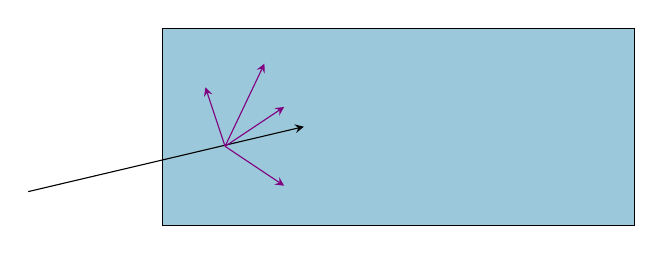
\begin{tikzpicture}
      \draw[fill=cyan!50!gray!60!] (-1,-1.25) -- (-1,1.25) -- (5,1.25) -- (5,-1.25) -- cycle;
      %frecce
      \draw[-stealth] (-2.7,-0.825) -- (0.8,0);
      \draw[-stealth,violet] (-0.2,-0.25) -- (-0.45,0.5);
      \draw[-stealth,violet] (-0.2,-0.25) -- (0.3,0.8);
      \draw[-stealth,violet] (-0.2,-0.25) -- (0.55,0.25);
      \draw[-stealth,violet] (-0.2,-0.25) -- (0.55,-0.75);
    \end{tikzpicture}
\end{figure}

Quando una particella attraversa lo scintillatore, i fotoni di scintillazione prodotti vengono emessi in tutte le direzioni, per cui se se non ricoprissimo le pareti dello scintillatore con qualche materiale nel momento in cui i fotoni raggiungono il bordo dello scintillatore essi subirebbero rifrazione e fuoriuscirebbero, e ciò significherebbe perderli.\footnote{Piccola curiosità: la prof La Rocca lavorò col padre di Marco Russo, il quale diceva sempre che "I fotoni sono bastardi" perché escono e anche una leggerissima crepa nella copertura comporta delle perdite notevoli in termini di raccolta della luce.}

Emergono quindi due necessità:

\begin{enumerate}[leftmargin=0.6cm]
   \item Cercare di evitare che questi fotoni fuoriescano dal rivelatore;
   \item Cercare di convogliare i fotoni in una piccola regione dove andiamo a posizionare il fotosensore.
\end{enumerate}

Quello che si fa tipicamente è rivestire le pareti dello scintillatore con un materiale possibilmente riflettente eccetto la parete/la zona dove si va a posizionare il fotosensore:

\begin{figure}[H]
   \centering
   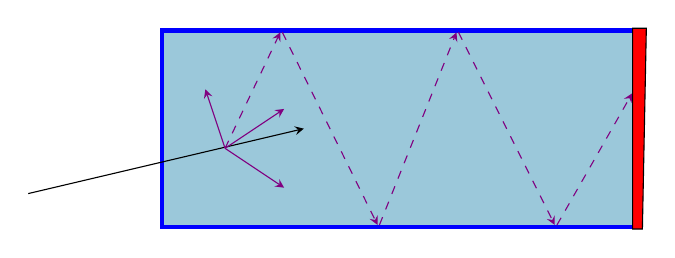
\begin{tikzpicture}
      \draw[line width=0.6mm, blue, fill=cyan!50!gray!60!] (-1,-1.25) -- (-1,1.25) -- (5,1.25) -- (5,-1.25) -- cycle;
      %frecce
      \draw[-stealth] (-2.7,-0.825) -- (0.8,0);
      \draw[-stealth,violet] (-0.2,-0.25) -- (-0.45,0.5);
      \draw[-stealth,violet] (-0.2,-0.25) -- (0.55,0.25);
      \draw[-stealth,violet] (-0.2,-0.25) -- (0.55,-0.75);
      %freccia dashed
      \draw[-stealth,dashed,violet,shorten >= 0.3mm] (-0.2,-0.25) -- (0.514,1.25);
      \draw[-stealth,dashed,violet,shorten <= 0.3mm, shorten >= 0.3mm] (0.514,1.25) -- (1.75,-1.25);
      \draw[-stealth,dashed,violet,shorten <= 0.3mm, shorten >= 0.3mm] (1.75,-1.25) -- (2.75,1.25);
      \draw[-stealth,dashed,violet,shorten <= 0.3mm, shorten >= 0.3mm] (2.75,1.25) -- (4,-1.25);
      \draw[-stealth,dashed,violet,shorten <= 0.3mm, shorten >= 0.6mm] (4,-1.25) -- (5,0.5);
      %fotosensore
      \draw[ fill=red] (5.1,-1.275) -- (5.15,1.275) -- (4.975,1.275) -- (4.975,-1.275) -- cycle;
    \end{tikzpicture}
\end{figure}

La copertura degli scintillatori non serve quindi soltanto per proteggerlo dall'umidità, ma anche per permettere alla luce di essere riflessa in modo da arrivare al fotosensore.

Oltre che tramite l'uscita attraverso i bordi dello scintillatore, si può avere una perdita di luce anche attraverso l'assorbimento da parte del materiale dello scintillatore, la quale è detta self-absorption. Quest'ultimo effetto è rilevante quando le dimensioni del rivelatore sono tali che le lunghezze totali dei cammini percorsi dai fotoni sono paragonabili alla lunghezza di attenuazione, la quale è un parametro definito come quella lunghezza dopo la quale l'intensità luminosa è ridotta di un fattore $e^{-1}$. L'intensità luminosa in funzione della lunghezza percorsa è quindi:

\begin{equation*}
   L(x)=L_0 e^{-x/\lambda}
\end{equation*}

dove $\lambda$ è la lunghezza di attenuazione, $x$ è la lunghezza del cammino percorso dalla luce e $L_0$ l'intensità luminosa iniziale. Poiché una tipica lunghezza di attenuazione è dell'ordine di 1 m o più, è chiaro che solo i rivelatori molto grandi ne sono influenzati. Bisogna comunque stare attenti perché chiaramente, in base allo schema visto sopra, i fotoni potrebbero percorrere tramite le riflessioni spazi molto lunghi e quindi alla fine essere assorbiti anche in rivelatori piccoli.

Inoltre potremmo avere anche effetti di assorbimento nelle pareti, cioè il materiale introdotto per avere riflessione potrebbe essere soltanto parzialmente riflettente e quindi c'è una piccola probabilità che un fotone venga assorbito anziché essere riflesso. Per quantificare tale effetto si definisce il coefficiente di riflettività, il quale va da 0 a 1 e che stabilisce la probabilità di avere riflessione o assorbimento.% Un materiale che viene spesso adoperato per rivestire le pareti di uno scintillatore è il Mylar.

\vspace{0.2cm}Fino ad ora abbiamo immaginato che la riflessione fosse perfettamente speculare\footnote{La riflessione speculare consiste nella riflessione osservata quando un singolo raggio incidente che forma un angolo $\vartheta_i$ con la normale produce un singolo raggio riflesso con angolo $\vartheta_r$ rispetto alla normale con il verificarsi dell'uguaglianza $\vartheta_i=\vartheta_r$.}. A volte però si preferisce utilizzare dei materiali che provocano riflessione diffusa piuttosto che speculare, i quali tipicamente hanno una superficie rugosa. Ciò deriva dal fatto che, poiché la superficie non è perfettamente piana, l'angolo di incidenza dipenderà dall'inclinazione del particolare punto che viene colpito, causando uno schema molto più disordinato rispetto ad una riflessione speculare.

\begin{figure}[H]
   \centering
   \includegraphics[width=\textwidth]{immagini/riflessione_speculare.png}
   \caption*{Riflessione speculare.}
\end{figure}
\begin{figure}[H]
   \centering
   \includegraphics[width=\textwidth]{immagini/riflessione_diffusa.png}
   \caption*{Riflessione diffusa.}
\end{figure}

A volte vengono utilizzati dei materiali diffusivi come vernici bianche, ma anche sostanze come il biossido di titanio o il teflon. Il motivo è che un materiale bianco produce diffusione, dunque può andare bene per il nostro scopo. 

\subsection{Un esercizio di simulazione}
%Come abbiamo detto, uno dei problemi che possiamo avere è che questi fotoni possono percorrere anche spazi molto grandi, con la conseguenza di poter perdere fotoni perché potrebbero venire assorbiti. Ciò purtroppo ha anche delle conseguenze sulla risoluzione temporale: infatti finora ci siamo concentrati solo sui tempi di emissione di questa luce, che abbiamo detto sono tempi molto brevi, ma a questo punto il problema è anche raccogliere la luce e se la luce deve percorrere spazi lunghi è chiaro che il segnale che viene raccolto al fotosensore chiaramente può anche essere caratterizzato da tempi più lunghi di quelli che abbiamo visto fino ad ora.

Come abbiamo detto, uno dei problemi che possono insorgere è che questi fotoni potrebbero percorrere distanze molto grandi, con il rischio di perderne alcuni a causa dell'assorbimento. Questo purtroppo ha delle conseguenze anche sulla risoluzione temporale: finora ci siamo concentrati solo sui tempi di emissione della luce, che sono molto brevi, ma ora diventa importante anche il processo di raccolta. Se la luce deve percorrere lunghe distanze, è evidente che il segnale raccolto dal fotosensore potrebbe essere caratterizzato da tempi più lunghi rispetto a quelli considerati finora.

Bisogna allora stimare tale lunghezza percorsa. Per fare ciò possiamo realizzare una simulazione come segue: presa una regione di piano (ad esempio un rettangolo), estraiamo un punto a caso distribuito uniformemente dentro l'area del rettangolo, una direzione casuale (tra $0$ e $360^{\circ}$) e facciamo propagare un raggio luminoso che per semplicità assumiamo muoversi con velocità $v=c$, facendolo riflettere specularmente sulle pareti finché non arriva sul fotosensore. Dopodiché stimiamo in ciascun evento la lunghezza della traccia e costruiamo la distribuzione dei tempi impiegati a percorrere tale distanza. 

\begin{figure}[H]
   \centering
   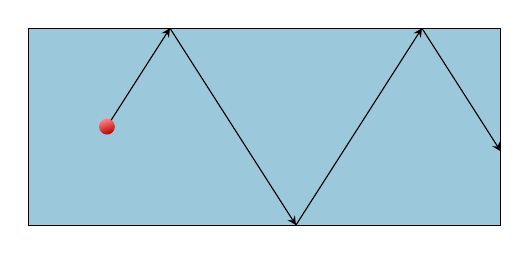
\begin{tikzpicture}
      \draw[fill=cyan!50!gray!60!] (-1,-1.25) -- (-1,1.25) -- (5,1.25) -- (5,-1.25) -- cycle;
      \draw[-stealth] (0,0) -- (0.8,1.25);
      \draw[-stealth] (0.8,1.25) -- (2.4,-1.25);
      \draw[-stealth] (2.4,-1.25) -- (4,1.25);
      \draw[-stealth] (4,1.25) -- (5,-0.3125);
      \shade[top color=red!50,bottom color=red!70!black,shading angle=20] (0,0) circle (0.1cm);
   \end{tikzpicture}
\end{figure}

\E chiaro che idealmente, se il fotone si muovesse verso il fotosensore, avremmo tempi abbastanza brevi perché se ad esempio il rivelatore fosse lungo 30 centimetri impiegheremmo un nanosecondo a raccogliere tutta la luce. Nella realtà non è così: a seguito di queste riflessioni le distanze percorse possono essere molto diverse, per cui abbiamo una distribuzione delle distanze percorse e quindi una distribuzione dei tempi necessari a percorrerle. Questo rappresenta un problema soprattutto quando il rivelatore ha geometrie particolari come ad esempio nel caso di bacchette di scintillatori, delle barre molto lunghe con una sezione piccola. Ecco perché in realtà ottimizzare un rivelatore di questo tipo risulta essere una procedura ostica, in quanto sebbene i processi di base siano semplici, a causa del comportamento dei fotoni si rischia di avere dei segnali troppo deboli.

%, quindi di raccogliere pochi fotoni da decine di migliaia di fotoni che possono essere prodotti però ogni web alla fine se ne raccolgono qualche decina, cioè immaginate quante perdite si hanno in tutti questi processi e

Quello che si può fare è studiare il comportamento del rivelatore e la raccolta di luce con dei simulatori professionali come ad esempio il simulatore GEANT4, il quale permette di seguire e di trasportare la luce nei materiali. 

Se volessimo realizzare una simulazione in cui seguiamo il percorso dei diversi fotoni che vengono prodotti per scintillazione in un rivelatore, dovremmo definire tantissime informazioni, ad esempio dovremmo specificare:

\begin{itemize}
   \item che tipo di luce viene emessa per scintillazione, quindi lo spettro di emissione dello scintillatore;
   \item il tempo di decadimento, quindi quanto tempo si impiega a emettere questa luce;
   \item l'assorbimento del materiale stesso, quantificato attraverso un coefficiente di assorbimento;
   \item le proprietà di riflessione del materiale che abbiamo posto sulle pareti;
   \item effetti di rifrazione quando si passa da un mezzo a un altro;
   \item il tipo di superficie di rivestimento, cioè se è una superficie perfettamente liscia o scabra;
   \item processi di scattering della luce e altri tipi di processi.
\end{itemize}

\begin{esempio}
   Con tale simulatore è possibile studiare la riflettività ad opera della superficie alluminizzata (cioè riflettente) nel caso in cui essa sia dipendente dalla lunghezza d'onda anziché costante. L'andamento che si osserva è il seguente:
   \begin{figure}[H]
      \centering
      \includegraphics[width=0.6\textwidth]{immagini/andamento_riflettività.png}
   \end{figure}
   In particolare, notiamo che per la riflessione di luce emessa da uno scintillatore (quindi tipicamente sui 400 nanometri), il coefficiente di riflettività varia parecchio, scendendo anche all'83-85\%, fatto che è importante da tenere in conto perché cambiano notevolmente le prestazioni del rivelatore.
\end{esempio}

\begin{esempio}
   Supponiamo di avere delle barre di lunghezza 1 m e di sezione all'incirca $1 \; \rm cm^2$ e di voler studiare il percorso della luce all'interno di questa barra con l'idea di raccogliere la luce all'estremità, quindi la luce che viene prodotta deve percorrere anche distanze di decine di centimetri per arrivare all'estremità in base a dove è stata prodotta, dunque a dove è passata la particella. Il grafico del numero di fotoni che riescono a percorrere una data distanza in base alle caratteristiche del rivelatore è il seguente:
   \begin{figure}[H]
      \centering
      \includegraphics[width=0.65\textwidth]{immagini/grafico_numero_fotoni.png}
   \end{figure}
   Nel grafico abbiamo due condizioni diverse di riflettività (90\% e 80\%) e due condizioni diverse di superficie, levigata o rugosa. Per entrambi i tipi di superficie, a seguito dell'assorbimento il numero di fotoni diminuisce esponenzialmente (da notare che la scala delle ordinate è logaritmica), mentre l'effetto della riflettività dipende dal tipo di superficie. In particolare, se la superficie è polished, cioè levigata, possiamo notare come la riflettività incida sensibilmente, tant'è che le due curve per i due regimi sono nettamente separate, mentre nel caso di superficie rugosa gli effetti di riflettività contano di meno ma rispetto alla superficie levigata abbiamo una notevole diminuzione dei fotoni.
   
   In questo modo otteniamo delle indicazioni attraverso le simulazioni anziché sperimentalmente, dunque possiamo poi passare all'apparato sperimentale soltanto per verificare quanto trovato.
\end{esempio}

\subsection{Guide di luce}

A volte può essere utile realizzare delle guide di luce, ovvero oggetti in plexiglass che facilitano l'accoppiamento tra lo scintillatore e il fotosensore. Questi due elementi potrebbero infatti avere geometrie differenti, oppure potrebbe essere necessario posizionare il rivelatore all'interno di un campo magnetico mentre il fotosensore, a causa delle sue caratteristiche, non può funzionare in tale ambiente. Il motivo è che il fotosensore potrebbe sfruttare campi elettrici o il movimento di particelle cariche che risentirebbero negativamente della presenza del campo magnetico. In questi casi, è necessario spostare il sensore fuori dal campo magnetico.

\begin{figure}[H]
   \centering
   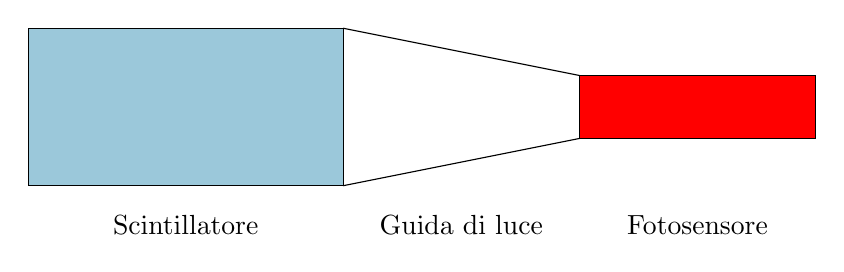
\begin{tikzpicture}
      \draw[fill=cyan!50!gray!60!] (-1,-1) -- (-1,1) -- (3,1) -- (3,-1) -- cycle;
      \draw (3,1) -- (6,0.4);
      \draw (3,-1) -- (6,-0.4);
      \draw[fill=red] (6,-0.4) -- (6,0.4) -- (9,0.4) -- (9,-0.4) -- cycle;
      \node at (1,-1.5) {Scintillatore};
      \node at (4.5,-1.5) {Guida di luce};
      \node at (7.5,-1.5) {Fotosensore};
   \end{tikzpicture}
\end{figure}

%A volte può tornare utile realizzare delle guide di luce, cioè degli oggetti realizzati in plexiglass che permettano un accoppiamento più agevole tra lo scintillatore e il rivelatore, in quanto quest'ultimi potrebbero avere geometrie diverse oppure potrebbe accadere che il rivelatore si trovi dentro un campo magnetico ma il fotosensore per qualche motivo non può lavorare all'interno di un campo magnetico, perché magari sfrutta dei campi elettrici, dei moti di particelle cariche che all'interno di un campo magnetico vengono sconvolte, quindi bisogna portare il sensore fuori dal campo magnetico.

Queste guide trasportano dunque la luce verso il fotosensore. Tuttavia, ogni componente che aggiungiamo comporta perdita di fotoni. Come infatti si evince anche dalla figura sopra, non possiamo prendere tutti i fotoni e trasportarli su una superficie più piccola, perché in un certo senso il flusso di fotoni non è comprimibile, cioè non valgono le stesse regole che valgono ad esempio nel trasporto dei fluidi in un condotto, dove vale la conservazione della massa: qui al massimo possiamo trasportare una quantità di luce che è proporzionale al rapporto tra area del fotosensore e area dello scintillatore:
\begin{equation*}
   F=\frac{A_{\rm fotosensore}}{A_{\rm scintillatore}}
\end{equation*}
L'idea alla base delle guide di luce è quella di cercare di guidare il più possibile la luce attraverso delle geometrie opportune che facilitino il fenomeno della riflessione totale. Ci sono geometrie molto varie, esempi di geometrie in cui si accoppia uno scintillatore avente sezione rettangolare con un fotosensore di forma cilindrica sono i seguenti:
\begin{figure}[H]
   \centering
   \includegraphics[width=\textwidth]{immagini/guide_di_luce.png}
\end{figure}
\subsection{Fibre WLS}
Nel caso in cui lo scintillatore abbia la forma di una lunga barra, dove posizioniamo il fotosensore? Potremmo pensare di posizionarlo agli estremi della barra, però ciò prevede che la luce venga trasportata fino all'estremità e abbiamo visto che c'è una notevole perdita di luce a seguito di diversi effetti. Un'alternativa potrebbe essere quella di utilizzare delle particolari fibre ottiche chiamate WaveLength Shifter fibers o fibre WLS. Esse sono delle fibre che assorbono un determinato range di lunghezze d'onda e lo riemettono a una lunghezza d'onda tipica, cioè spostano la lunghezza d'onda della luce. La loro caratteristica è che assorbono anche la luce che incide lateralmente.

Prima di parlare di queste, vediamo com'è composta una fibra ottica:
\begin{figure}[H]
   \centering
   \includegraphics[width=0.65\textwidth]{immagini/struttura_fibra_ottica.png}
\end{figure}
Essa è costituita da due cilindri concentrici, di cui il più interno prende il nome di core e costituisce il cuore della fibra con un determinato indice di rifrazione, mentre quello più esterno che circonda il primo prende il nome di cladding, che ha un diverso indice di rifrazione. Tali materiali sono tali che l'indice di rifrazione della parte interna è maggiore rispetto a quella della parte esterna: ciò fa sì che se la luce entra con un'opportuna angolazione può essere guidata attraverso la fibra ottica mediante riflessioni totali, la quale è permessa solamente se si passa da un indice di rifrazione maggiore a uno minore. Quindi l'idea è riuscire a guidare la luce anche in percorsi non rettilinei (dunque curvati) attraverso queste riflessioni totali.

Quello appena descritto è il principio di funzionamento della normale fibra ottica. La fibra WLS è un po' diversa perché la fibra ottica può trasportare la luce solamente se questa entra dalla sezione: in tal caso essa verrà guidata e uscirà dall'altro lato, mentre una luce che incide lateralmente non riesce ad entrare nella fibra perché subisce rifrazione e fuoriesce. Questa fibra invece ha la caratteristica di assorbire la luce, quindi anche la luce che incide lateralmente viene assorbita e poi riemessa alla lunghezza d'onda caratteristica. La luce che viene riemessa, siccome si trova all'interno della fibra, in automatico viene guidata verso l'esterno. Tale principio di funzionamento risulta molto utile, perché se distendiamo tale fibra all'interno dello scintillatore, essa sarà in grado di assorbire la luce emessa dallo scintillatore in quanto la luce colpirà la fibra lungo tutta la sua superficie esterna, riemettendola e quindi guidandola verso l'esterno, e a quel punto possiamo collegare un fotosensore all'esterno della fibra.

Come facciamo a incapsulare la fibra all'interno di una barra? Ci sono diverse tecniche, a volte con la tecnica dell'estrusione si può realizzare una barra che presenta al centro un foro dove far passare la fibra ottica, oppure sempre per estrusione si realizza una barra che presenta un solco sulla superficie su cui si posiziona la fibra ottica. Questa è una tecnica molto utile quando si ha a che fare con degli scintillatori di dimensioni molto estese, dove diventa difficile avere fotosensori estesi, quindi o si mettono tanti fotosensori che si devono far lavorare in coincidenza ma diventa complicato oppure si va a posizionare una fibra ottica WLS così da raccogliere la luce attraverso essa e il fotosensore si posiziona all'estremità delle fibra ottica. Ciò è molto utile anche perché se ad esempio abbiamo due estremità possiamo posizionare solamente due rivelatori, li mettiamo in coincidenza (cioè si fa in modo che misuriamo solamente quando entrambi danno un segnale) perché se viene prodotta la luce e si incanala nella fibra ottica andrà verso entrambe l'estremità, quindi ci aspettiamo un segnale da entrambe le estremità e questo ci permette di ridurre gli eventi di rumore di fondo perché è improbabile che si abbia una coincidenza. 

Per quanto riguarda lo spettro di assorbimento e quello di emissione, essi devono essere diversi: lo spettro di assorbimento si deve adattare allo scintillatore, quindi deve essere verso l'UV, lo spettro di emissione si deve adattare al fotosensore, il quale deve vedere questa luce.

\begin{figure}[H]
   \centering
   \includegraphics[width=0.6\textwidth]{immagini/spettro_emissione_assorbimento_fibre_WLS.png}
\end{figure}

%sono molto utili quando si adoperano dei rivelatori di grandi superfici, quindi dei rivelatori in cui la luce viene prodotta su una superficie molto estesa e quindi bisognerà andare a ricoprire in diversi punti la superficie con dei fotosensori per essere sicuri di poter raccogliere tutta la luce prodotta e avere un'efficienza abbastanza uniforme del nostro rivelatore.

%immaginate ad esempio di avere un rivelatore delle superfici di questo tavolo è chiaro che se io nasse ad accoppiare un solo fotosensore magari a un estremità di questo di questo tavolo è chiaro che la luce prodotta all'altra estremità potrebbe essere persa perché i fotoni dovrebbero arrivare attraverso diverse riflessioni verso il mio fotosensore quindi avrei un'efficienza non uniforme magari riesco a vedere bene le particelle che deposita una energia in prossimità del fotosensore ma tutta l'altra zona del mio rivelatore potrebbe presentare efficienza abbastanza bassa 

\section{Rivelatori basati su scintillatori}
I rivelatori basati su scintillatori vengono impiegati in diversi campi della fisica: fisica nucleare, astroparticellare, ma anche fisica applicata, in particolare nel campo medico.

%ad esempio nel campo della ricerca fisica in ambito nucleare e astroparticellare, oppure ad esempio per la costruzione di calorimetri, rivelatori in grado di misurare l'energia di una particella oppure rivelatori per raggi cosmici ma anche nel campo della fisica applicata.

%vedremo anche qui alcuni esempi o applicazioni mediche qui vediamo non ve l'ho portato ma con quello vedrete poi in laboratorio un tipico esempio di un fotomoltiplicatore appoppiato una scintillatore anzi ne ho portato una volta scorso effettivamente io avevo detto appunto che lo scintillatore era solamente una porzione di quello che vedevate tutti il resto che cos'era era una guida di luce è un fotomoltiplicatore che questo caso era il fotosensore quindi tipicamente voi vedrete sempre uno scintillatore insieme un fotosensore che può essere più o meno meno a seconda del tipo di fotosensore che è stato scelto quindi in questo caso questa parte cilindrica a destra costituisceisci lo scintillatore accoppiato a un fotomoltiplicatore che vedete sulla sinistra di cui parleremo breve chiaramente si possono anche realizzare delle strutture che comprendono più scintillatori quindi ad esempio ad esempio esempio degli array come quello mostrato in figura dove abbiamo tanti scintillatori che puntano verso una ben precisa porzione di spazio, dove magari avviene una reazione da cui vengono emesse delle particelle, quindi si realizza una corona di rivelatori, in questo caso di scintillatori, che circondano il punto di interazione analogamente. Qui vedete, siccome sono dei materiali, come vi ho detto, che possono essere lavorati facilmente, possono anche assumere delle forme caratteristiche adatte al tipo di misura che si deve effettuare. Poi ogni scintillatore ovviamente ha associato al suo fotomoltiplicatore, quindi quindi sono tantissime geometrie possibili. 

\subsection{Un esempio di applicazione: la PET}
Gli scintillatori vengono adoperati in esami diagnostici come la PET, la Positron Emission Tomography. Quest'esame diagnostico consiste nell'andare a misurare dei raggi $\gamma$ che vengono emessi da un determinato punto e vengono emessi in coincidenza, cioè vengono emessi simultaneamente in direzione opposte.

Lo scopo della PET consiste nell'individuare l'eventuale presenza di cellule cancerogene, che sono tipicamente delle cellule che hanno un elevato consumo di glucosio. Nel paziente viene quindi iniettato un liquido che contiene del glucosio e un elemento tracciante, cioè un isotopo che tipicamente emette dei positroni e una volta emessi questi si annichilano e danno un luogo a due $\gamma$ identici emessi a $180^{\circ}$.
\begin{figure}[H]
   \centering
   \includegraphics[width=0.6\textwidth]{immagini/pet_1.png}
\end{figure}
Questo tracciante si concentra nelle zone ad alto metabolismo e quindi andando a ricostruire questi $\gamma$ che vengono emessi si possono individuare delle zone dove c'è una maggiore emissione, quindi dove si è andato a concentrare questo tracciante. Chiaramente per ricostruire due $\gamma$ a $180^{\circ}$ bisogna avvolgere in qualche modo con una corona di rivelatori il paziente, quindi in una PET tipicamente si presentano delle strutture ad arco che sono costituite da scintillatori in grado di misurare questi $\gamma$ in maniera tale che quando si osserva un segnale in coincidenza, quindi un segnale in una coppia di scintillatori opposti simultaneamente si può andare a ricostruire quella che è la direzione di arrivo dei $\gamma$ e andando a tracciare tutti questi $\gamma$ si può andare a individuare la sorgente da cui vengono emessi questi $\gamma$.
\begin{figure}[H]
   \centering
   \includegraphics[width=0.7\textwidth]{immagini/pet_2.png}
\end{figure}
Nelle PET tradizionali di prima generazione questi scintillatori erano accoppiati a fotomoltiplicatori, dei fotosensori che avevano però lo svantaggio di non poter lavorare all'interno di campi magnetici, il che è limitante. Per questo motivo si è pensato di sostituire i fotomoltiplicatori con nuovi fotosensori di ultima generazione basati su materiali a stato solido.